\documentclass[10pt]{beamer}

\usepackage[style=numeric, sorting=none]{biblatex}
\addbibresource{demo.bib}
\setbeamertemplate{bibliography item}{\insertbiblabel}

\usetheme[progressbar=frametitle, titleformat=smallcaps]{metropolis}
\usepackage{appendixnumberbeamer}
\usepackage{booktabs}
\usepackage[scale=2]{ccicons}
\usepackage{pgfplots}
\usepackage{xcolor}
\definecolor{Purple}{RGB}{51, 0, 111}
\definecolor{Orange}{RGB}{232, 211, 162}
\setbeamercolor{normal text}{fg=black,bg=white}
\setbeamercolor{palette primary}{fg=Orange, bg=Purple}
\definecolor{Indigo}{rgb}{0.29, 0.0, 0.51}
\definecolor{Jade}{rgb}{0.0, 0.66, 0.42}
\setbeamercolor{alerted text}{fg=Orange}
\setbeamercolor{frametitle}{bg=Purple, fg=Orange}

\usepackage{forest}
\usepackage{soul}
\usepgfplotslibrary{dateplot}
\usepackage{xspace}
\newcommand{\themename}{\textbf{\textsc{metropolis}}\xspace}
\usepackage{tikz}
\usepackage[default,scale=0.95]{opensans}
\usepackage[T1]{fontenc}
\usepackage[printwatermark]{xwatermark}

%title slide information
\title{Racial Disparity in Exposure to Housing Cost Burden in the U.S.: 1980-2017}
\date{}
\author{Chris Hess$^1$, Gregg Colburn$^2$, Kyle Crowder$^1$, Ryan Allen$^3$}
\institute{$^1$ University of Washington, Department of Sociology \\ $^2$ University of Washington, Runstad Department of Real Estate \\ $^3$ University of Minnesota, Humphrey School of Public Affairs}
\titlegraphic{\hfill
\includegraphics[height=1cm]{W-Logo_Purple_RGB.png}}

\begin{document}

%title slide
\maketitle

%what is housing cost burden, how does this applied concept intersect with racial inequalities in housing?
\begin{frame}{Introduction}
\setbeamercolor{normal text}{fg=lightgray,bg=}
\setbeamercolor{alerted text}{fg=black,bg=}
\usebeamercolor{normal text}
\begin{itemize}
    \onslide<1->{\alert<+>{\item Existing scholarship notes material racial disparities in housing access, housing quality, and neighborhood conditions.}}
    \onslide<2->{\alert<+>{\item For example, research on residential attainment has consistently observed black-white inequality in households' likelihood of moving into and out of high-poverty neighborhoods \cite{south1997escaping} \cite{crowder2005race}.}}
    \onslide<3->{\alert<+>{\item Socioeconomic disadvantages related to neighborhood context and rising housing costs both contribute to a given households' likelihood of experiencing economic hardship.}}
    \onslide<4>{\alert<+>{\item Housing cost burden was the most frequently reported economic challenge in a recent Urban Institute study \cite{karpman2019despite}.}}
\end{itemize}
\end{frame}

%why is this important to study?
\begin{frame}{Introduction}
\setbeamercolor{normal text}{fg=lightgray,bg=}
\setbeamercolor{alerted text}{fg=black,bg=}
\usebeamercolor{normal text}
\begin{itemize}
    \onslide<1->{\alert<+>{\item The Joint Center for Housing Studies' \textit{State of the Nation’s Housing} series, documents significant and persistent racial disparities in the prevalence of housing cost burden \cite{jchs2019state}.}}
    \onslide<2->{\alert<+>{\item An important open question is  whether this black-white gap persists after adjusting prevalence estimates for characteristics of households and broader contexts that are salient to both household income and typical housing costs.}}
    \onslide<3->{\alert<+>{\item Given serious consequences like constrained expenditures on other necessities, it is important for housing researchers and practitioners to understand what factors contribute to elevated risk and racial inequality in exposure to housing cost burden.}}
\end{itemize}
\end{frame}

%what do we do in this study?
\begin{frame}{Research Questions}
\begin{itemize}
    \item In this paper, we focus on the following research questions:
    \begin{enumerate}
        \item How has the black-white disparity in housing cost burden changed over time?
        \item To what extent do household characteristics, neighborhood context, and metropolitan location explain the racial disparities in income and housing cost that drive patterns of housing cost burden?
    \end{enumerate}
\end{itemize}
\end{frame}

%what existing research is there on racial inequalities in housing?
\begin{frame}{Background}
\setbeamercolor{normal text}{fg=lightgray,bg=}
\setbeamercolor{alerted text}{fg=black,bg=}
\usebeamercolor{normal text}
\begin{itemize}
    \onslide<1->{\alert<+>{\item Both the cost of housing (numerator) and the household income (denominator) have an independent effect on housing cost burden.}}
    \onslide<2->{\alert<+>{\item Wages stagnated over past decades, particularly among the bottom half of the income distribution. \cite{mishel2015wage}.}}
    \onslide<3->{\alert<+>{\item Residential segregation creates racial inequality in exposure to high levels of neighborhood poverty, which has important implications for educational attainment and upward socioeconomic mobility \cite{massey1993american} \cite{quillian2012segregation}.}}
    \onslide<4>{\alert<+>{\item Continued racial disparities in HH income resources related to segregation are a key factor contributing to racial inequality in exposure to housing cost burden.}}
\end{itemize}
\end{frame}

%why are existing disadvantages relevant to HCB for different reasons?
\begin{frame}{Background}
\setbeamercolor{normal text}{fg=lightgray,bg=}
\setbeamercolor{alerted text}{fg=black,bg=}
\usebeamercolor{normal text}
\begin{itemize}
    \onslide<1->{\alert<+>{\item Variations in segregation between metropolitan areas also relevant to creating disparities in concentration of racial minorities in central city neighborhoods, some of which have experienced sharp increases in housing cost.}}
    \onslide<2->{\alert<+>{\item To the extent that white households may pay a premium to exercise a preference for segregation, metropolitan areas with higher degrees of segregation may also have higher prevalence of white households facing cost burden. \cite{cutler1999rise}.}}
    \onslide<3->{\alert<+>{\item Housing cost burden limits a household's capacity to weather unexpected expenses, invest in human capital, among other things.}}
\end{itemize}
\end{frame}

%what do we use for this study, why is the PSID useful
\begin{frame}{Data}
\setbeamercolor{normal text}{fg=lightgray,bg=}
\setbeamercolor{alerted text}{fg=black,bg=}
\usebeamercolor{normal text}
\begin{itemize}
    \onslide<1->{\alert<+>{\item Panel Study of Income Dynamics (PSID)
    \begin{itemize}
        \item Longitudinal survey of U.S. households
        \item Initial sample of 5,000 families, with the `PSID gene' following children of the original respondents
        \item Interviewed annually 1968-1997, then odd years 1999-2017
        \item Analyze interview waves from 1980-2017 (1980 is earliest Census for tract median rent)
        \item Subset to head of households who rent
        \item 32,164 renter HH observations
    \end{itemize}}}
    \onslide<2->{\alert<+>{\item Decennial Census + American Community Survey (ACS)
    \begin{itemize}
        \item Tract and CBSA measures of population and housing composition
        \item 1980, 1990, 2000, 2010, 2013-2017
        \item Linear interpolation for intercensal waves
    \end{itemize}}}
\end{itemize}
\end{frame}

%how do we define key measures used in our analysis?
\begin{frame}{Measures}
\textbf{RQ1:} Estimate difference in probability of exposure to housing cost burden among black and white HHs over time
\begin{table}
	\centering
\begin{tabular}{r|p{3.1in}}
	\onslide<1->{\textit{Cost Burden} & Ratio of rent payment to total family income >= .30} \\
	\onslide<1->{&  \scriptsize Housing expenditure does not include utilities since this variable was not consistently asked} \\
    \addlinespace
    \addlinespace
    \onslide<2->{\textit{Race} & Head of household's self-reported race} \\
    \onslide<2->{& \scriptsize Analysis focuses on black and white households because other racial/ethnic groups have small Ns, particularly early in panel} \\
    \addlinespace
    \addlinespace
    \onslide<3->{\textit{Time Period} & Wave fixed effects to assess temporal variation} \\
    \onslide<3->{& \scriptsize Reference period set to 1980} \\
\end{tabular}
\end{table}
\end{frame}

%how do we define our control measures
\begin{frame}{Measures}
\textbf{RQ2:} Adjust estimated probability of exposure to HCB using covariates relevant to housing cost or household resources.
\begin{table}
	\centering
\begin{tabular}{r|p{3.1in}}
	\onslide<1->{\textit{Household} & Age, sex, education, marital status/cohabitation, new HoH status, N in family, employment, whether supports outside dependents, N rooms in HU} \\
    \addlinespace
    \addlinespace
    \onslide<2->{\textit{Neighborhood} & Median gross rent, logged total population, poverty rate, prop. HU owner-occupied, prop. HU vacant, prop. HU SFH, prop. HU built >= 1970} \\
    \addlinespace
    \addlinespace
    \onslide<3->{\textit{Metropolitan} & Median gross rent, logged total population, prop. HU built >= 1970, black-white segregation (D)} \\
\end{tabular}
\end{table}
\end{frame}

%what methods do we use for analyzing HCB disparities over time?
\begin{frame}{Methods}
\begin{itemize}
    \onslide<1->{\item Logistic regression models stratified by head of household race}
    \onslide<2->{\item Nested model specifications:
    \begin{enumerate}
        \item Time fixed-effects
        \item + household composition
        \item + neighborhood composition
        \item + metropolitan composition
    \end{enumerate}}
    \onslide<3->{\item Standard errors clustered by household \cite{cameron2015practitioner}.}
    \onslide<4->{\item Marginal predictions and average marginal effects (AME) are the focus of the results section to facilitate comparability between models \cite{allison1999comparing}.
    \begin{itemize}
        \item Time-series graphics visualize odd-years to cope with plotting of factor variables at constant year interval
        \item Ropeladder graphics visualize AMEs for adjustment covariates, proportion measures show change from 0\% $\rightarrow$ 100\%
    \end{itemize}}
\end{itemize}
\end{frame}

%what are the basic trends over time in terms of housing cost burden by race
\begin{frame}{Results}
\vspace*{10pt}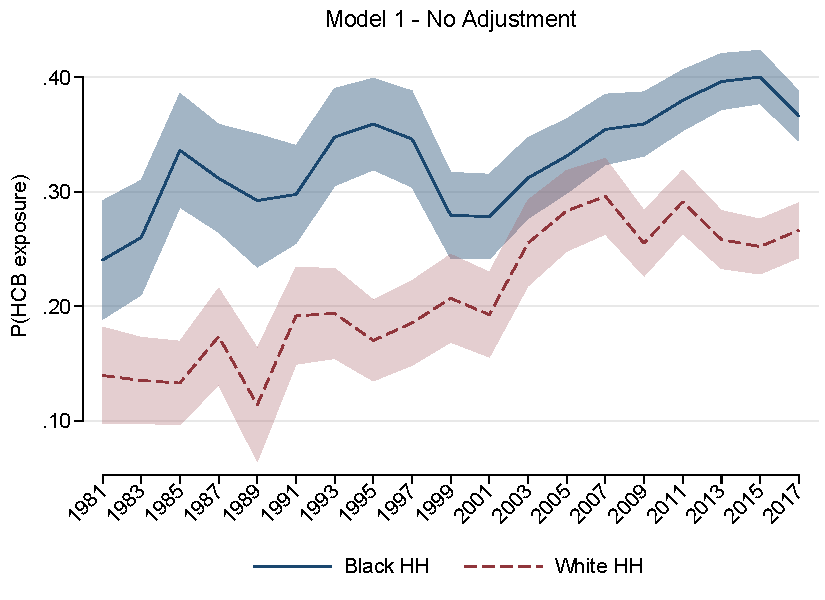
\includegraphics[width=\linewidth]{HCB_m1_ts.pdf}
\end{frame}

%how much can we account for using household-level composition differences?
\begin{frame}{Results}
\vspace*{10pt}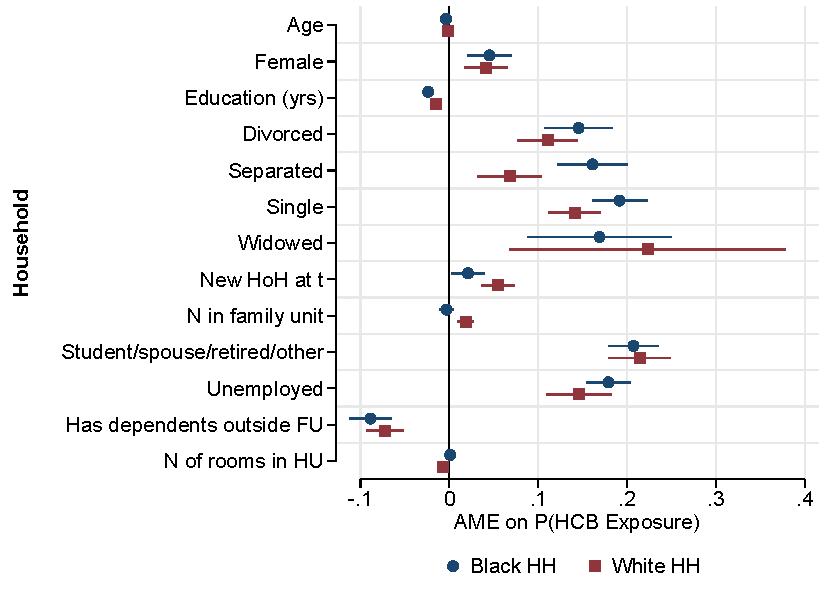
\includegraphics[width=\linewidth]{HCB_m2_ame_ropeladder.pdf}
\end{frame}

%how much can we account for using neighborhood-level composition differences?
\begin{frame}{Results}
\vspace*{10pt}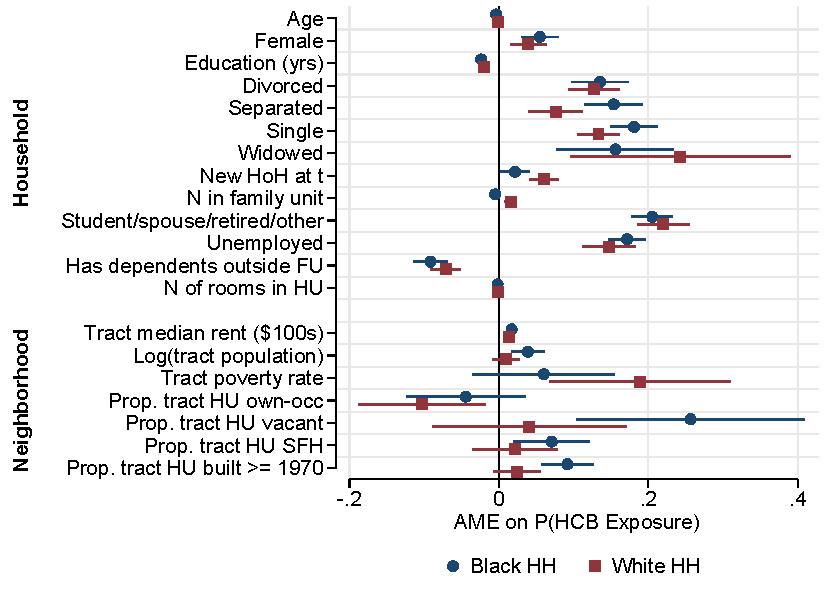
\includegraphics[width=\linewidth]{HCB_m3_ame_ropeladder.pdf}
\end{frame}

%how much can we account for using metro-level composition differences?
\begin{frame}{Results}
\vspace*{10pt}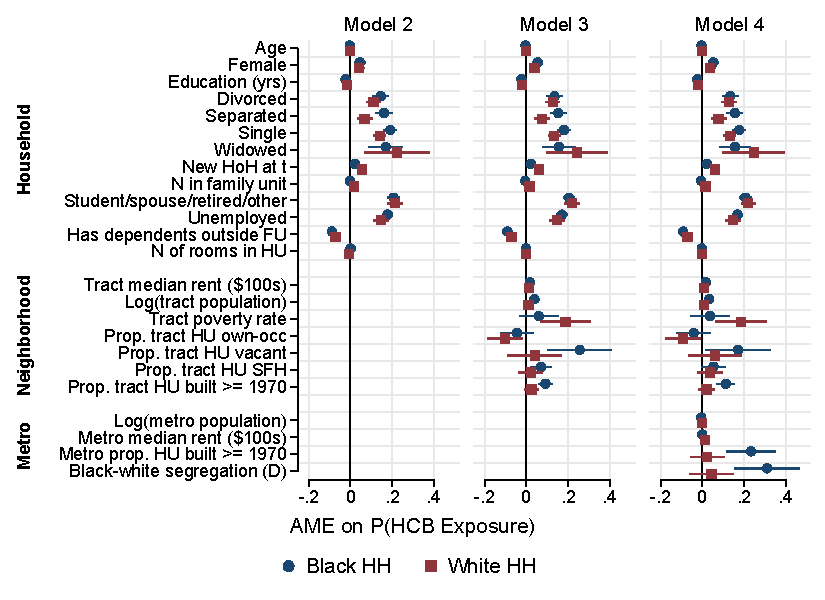
\includegraphics[width=\linewidth]{HCB_ame_ropeladder_mod_compare.pdf}
\end{frame}

%what do the fully-adjusted trends look like in terms of HCB exposure probability over time?
\begin{frame}{Results}
\vspace*{10pt}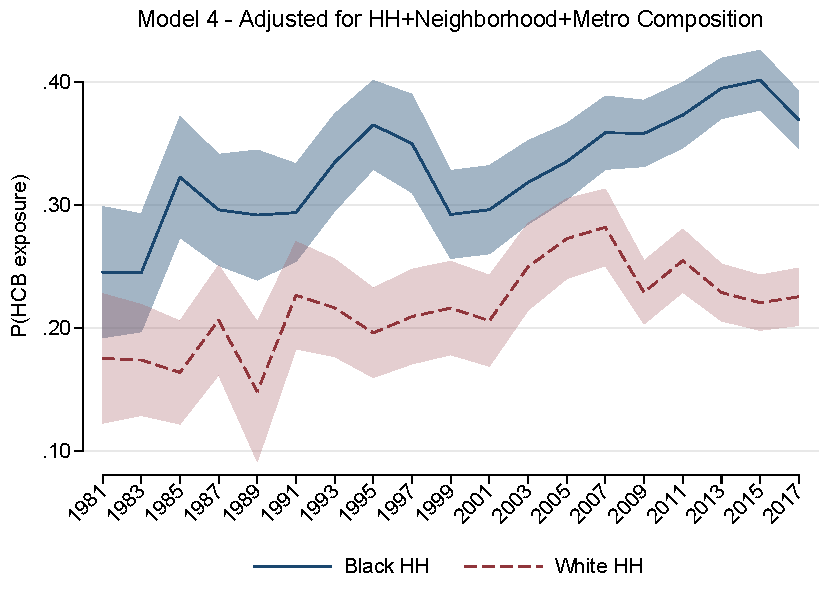
\includegraphics[width=\linewidth]{HCB_m4_ts.pdf}
\end{frame}

%review the main empirical takeaways
\begin{frame}{Discussion}
\setbeamercolor{normal text}{fg=lightgray,bg=}
\setbeamercolor{alerted text}{fg=black,bg=}
\usebeamercolor{normal text}
\begin{itemize}
    \onslide<1->{\alert<+>{\item Widening disparity long-term that remains unexplained after adjusting for many relevant household, neighborhood and metropolitan characteristics.}}
    \onslide<2->{\alert<+>{\item Able to explain most of change in white HH's exposure probability over time, but considerably less so for black HHs.}}
    \onslide<3->{\alert<+>{\item Housing crisis and recession relevant for longer-term change among black HHs, whereas recent change among white HHs largely accounted for.}}
    \onslide<4->{\alert<+>{\item Residential segregation and the age of the metropolitan housing stock create different pressures on HH relevant to greater racial inequality in HCB.}}
\end{itemize}
\end{frame}

%what limitations are important for us to note about the present analysis
\begin{frame}{Limitations}
\setbeamercolor{normal text}{fg=lightgray,bg=}
\setbeamercolor{alerted text}{fg=black,bg=}
\usebeamercolor{normal text}
\begin{itemize}
    \onslide<1->{\alert<+>{\item Household utility payments are not taken into account, this is pushing our exposure probability estimates downwards.}}
    \onslide<2->{\alert<+>{\item Since there is no tract rent estimate for 1970, we are unable to use the full span of PSID with valid geocodes (1970-2017).}}
    \onslide<3->{\alert<+>{\item Latino, Asian and other racial/ethnic groups have limited representation in the PSID, restricting our analysis to black and white households' trends in cost burden.}}
\end{itemize}
\end{frame}

%what directions / implications does our study have for future research on HCB?
\begin{frame}{Future Research}
\setbeamercolor{normal text}{fg=lightgray,bg=}
\setbeamercolor{alerted text}{fg=black,bg=}
\usebeamercolor{normal text}
\begin{itemize}
    \onslide<1->{\alert<+>{\item Investigate metropolitan-household interactions and intergenerational housing cost burden using PSID family structure.}}
    \onslide<2->{\alert<+>{\item Conduct spell analysis based on periods of exposure to housing cost burden.}}
    \onslide<3->{\alert<+>{\item Decompose cost burden inequality between black and white households into components related to income disparity and housing cost disparity.}}
\end{itemize}
\end{frame}

%close things up with a thank you
\begin{frame}[standout]
  \centering \Huge
  Thank You!
\end{frame}

%references
\begin{frame}[allowframebreaks]{References}
\printbibliography[heading=none]
\end{frame}

\end{document}
